%!TEX root = ../dokumentation.tex

\chapter{Implementierung}

\section{BaklavaJS}

Eine der Anforderungen war es, das Modell visuell bearbeiten zu können. Dafür war es notwendig, einen Graph-Editor zu entwickeln. Ein solcher Editor erlaubt es, Knoten hinzuzufügen bzw. zu entfernen und sie miteinander zu verbinden. Der Editor wurde als separate Bibliothek unter dem Namen \textit{BaklavaJS} entwickelt und ist somit auch für andere Projekte verwendbar.

Der Graph besteht aus Knoten und Kanten. Ein Knoten ist dabei wie eine mathematische Funktion: Er führt einen Algorithmus auf die Eingangsdaten aus und gibt die erzeugten Ausgangsdaten aus. Im Gegensatz zu einem "herkömmlichen" Graphen kann ein Knoten mehrere Kanten zu einem anderen Knoten haben.

Visuell wird ein Knoten in BaklavaJS folgendermaßen dargestellt:

\begin{figure}[H]
    \centering
    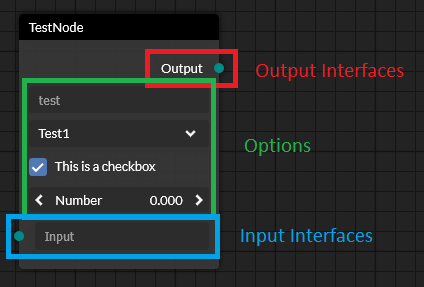
\includegraphics[width=.5\textwidth]{node_parts.png}
    \caption{Aufbau eines Knotens in BaklavaJS}
    \label{fig:nodeparts}
\end{figure}

Jeder Knoten besteht aus drei Teilen:
\begin{itemize}
    \item \textbf{Input Interfaces}: Die Eingangsschnittstellen eines Knotens werden benutzt, um Daten von anderen Knoten an diesen Knoten zu transferieren. Ist kein anderer Knoten verbunden, kann der Wert mittels eines Steuerelements auch direkt am Knoten eingestellt werden.
    \item \textbf{Options}: Hier können Werte eingestellt werden, die der Knoten für die Berechnung braucht, die aber beispielsweise zu komplex sind, um als Daten von anderen Knoten über Eingangsschnittstellen zu kommen.
    \item \textbf{Output Interfaces}: Die Ausgangsschnittstellen stellen das Ergebnis bereit, damit es von anderen Knoten benutzt werden kann.
\end{itemize}

\subsection{Ausführungsreihenfolge des Graphen}

\begin{figure}[H]
    \centering
    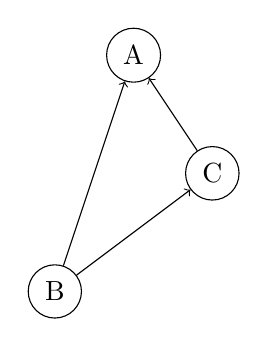
\begin{tikzpicture}
        \node[shape=circle,draw=black] (A) at (0,0) {A};
        \node[shape=circle,draw=black] (B) at (-1,-3) {B};
        \node[shape=circle,draw=black] (C) at (1,-1.5) {C};
        \path[->](B) edge node[left] {} (A);
        \path[->](B) edge node[left] {} (C);
        \path[->](C) edge node[left] {} (A);
    \end{tikzpicture}
    \caption{Beispielgraph}
    \label{fig:nodeExecutionOrder1}
\end{figure}

In Abbildung \ref{fig:nodeExecutionOrder1} ist ein Beispielgraph mit Knoten und Kanten zu sehen. Der Graph kann als Abhängigkeitsgraph interpretiert werden: Um den Knoten $A$ auszuführen, müssen vorher die Knoten $B$ und $C$ ausgeführt werden, damit die Ergebnisse dieser Knoten verfügbar sind. Auch muss der Knoten $B$ vor dem Knoten $C$ ausgeführt werden. $B$ hat keine Abhängigkeiten. Somit ergibt sich als Ausführungsreihenfolge $B \rightarrow C \rightarrow A$.

Die Ausführungsreihenfolge der Knoten muss folgende Bedingungen erfüllen:
\begin{itemize}
    \item Jeder Knoten wird genau einmal ausgeführt
    \item Ein Knoten kann erst ausgeführt werden, wenn alle Knoten, die Kanten zu ihm haben, ausgeführt wurden
\end{itemize}

\todo{Topological Sorting}

Topologische Sortierung kann nur auf azyklischen, gerichteten Graphen durchgeführt werden. Anhand des folgenden, zyklischen Graphen ist das leicht erkennbar:
\begin{figure}[H]
    \centering
    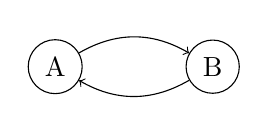
\begin{tikzpicture}
        \node[shape=circle,draw=black] (A) at (-1,0) {A};
        \node[shape=circle,draw=black] (B) at (1,0) {B};
        \path[->](A) edge[bend left] node[left] {} (B);
        \path[->](B) edge[bend left] node[left] {} (A);
    \end{tikzpicture}
    \caption{Zyklischer Graph}
    \label{fig:cyclicGraph}
\end{figure}
Knoten $B$ hat Knoten $A$ als Abhängigkeit. Somit muss Knoten $B$ vor Knoten $A$ ausgeführt werden. Allerdings hat $B$ den Knoten $A$ als Abhängigkeit. Es müsste somit der jeweils andere Knoten zuerst berechnet werden, was nicht möglich ist. Aus diesem Grund darf der Graph keine Zyklen enthalten.

\todo{JSPerf mit Kahn's algorithm vs custom algorithm}

Mit folgendem Algorithmus kann die Ausführungsreihenfolge bestimmt werden:
\begin{enumerate}
    \item Adjazenzliste erstellen
    \item Baum aufbauen mit Zykluserkennung
    \item Breitensuche um die Ausführungsreihenfolge zu bestimmen 
\end{enumerate}

\begin{algorithm}[H]
    \caption{Baum aufbauen mit Zykluserkennung}
    \begin{algorithmic}[1]
        \Function{findDescendants}{treeNode, ancestors, adjacency}
            \ForAll{$c$ in $treeNode.children$}
                \If{$c$ in $ancestors$}
                    \State Cycle detected
                \EndIf
                \State $ancestors.push(c)$
                \State $c.children = findChildren(c)$
                \State \Call{findDescendants}{c, ancestors, adjacency}
                \State $ancestors.pop()$
            \EndFor
        \EndFunction
    \end{algorithmic}
\end{algorithm}

\begin{algorithm}[H]
    \caption{Breitensuche um die Ausführungsreihenfolge zu bestimmen}
    \begin{algorithmic}[1]
        \State $queue \gets \textbf{new} \ Queue()$
        \State $stack \gets \textbf{new} \ Stack()$
        \State $queue.push(root)$
        \While{\textbf{not} $queue.isEmpty()$}
            \State $current \gets queue.dequeue()$
            \ForAll{$c$ in $current.children$}
                \State $stack.push(c)$
                \State $queue.enqueue(c)$
            \EndFor
        \EndWhile
        \State $calculationOrder \gets \textbf{new} \ List()$
        \While{\textbf{not} $stack.isEmpty()$}
            \State $current \gets stack.pop()$
            \If{\textbf{not} $calculationOrder.contains(current)$}
                \State $calculationOrder.append(current)$
            \EndIf
        \EndWhile
    \end{algorithmic}
\end{algorithm}

Am Beispiel des Graphen in Abbildung \ref{fig:nodeExecutionOrder1} sieht der Algorithmus folgendermaßen aus:

\todo{}

\subsection{Grafische Umsetzung}

\subsubsection{VueJS}
VueJS ist ein JavaScript Framework zum Erstellen von Browser-Frontends. Ein wichtiges Konzept in Vue sind \textit{Komponenten}. Komponenten sind kleine, eigenständige und wiederverwendbare UI-Elemente \cite{vue:components}.

In Anlehnung an das Model-View-Viewmodel-Pattern ist Vue \textit{reaktiv} gestaltet und bietet Datenbindung \cite{vue:instance}. Reaktiv bedeutet, dass Daten im sogenannten \textit{ViewModel} geändert werden können und diese Änderungen direkt in der \textit{View} angezeigt werden. \todo{Grafik zur Verdeutlichung}

Diese Art der Wiederverwendbarkeit ist essentiell, um die Knoten und Kanten zu zeichnen. Besonders hilfreich ist hierbei die \texttt{v-for}-Direktive. Sie erlaubt es, eine Liste von Komponenten zu rendern. Dabei werden Änderungen in der Liste über Datenbindung direkt in der UI übernommen. \todo{Mehr Erklärung}



\begin{itemize}
    \item Erklärung VueJS
    \item Wie werden die Kanten gezeichnet?
    \item Wie werden NodeOptions gezeichnet?
    \item Wie wird Zoom / Panning umgesetzt?
\end{itemize}

\subsection{Plugin-System und Event-System}

\subsection{BaklavaJS Pakete}
\begin{itemize}
    \item \textbf{Core}: Dieses Paket enthält alle notwendigen Klassen und Funktionen, um Knoten hinzuzufügen \todo{More}
    \item \textbf{Engine}: Erlaubt es, die Knoten in dem Graphen auszuführen und sorgt dafür, dass Daten über die Kanten übertragen werden
    \item \textbf{Interface-Types}: Fügt Typen zu Knoten-Schnittstellen hinzu. Standardmäßig können nur zwei Schnittstellen mit gleichem Typ miteinander verbunden werden. Es ist aber möglich, Ausnahmen anzugeben, sodass auch Schnittstellen unterschiedlichen Typs miteinander verbunden werden können. Dabei kann auch eine Konvertierungsfunktion mit angegeben werden. So kann zum Beispiel eine Number-Schnittstelle mit einer String-Schnittstelle verbunden werden. Die Konvertierungsfunktion wandelt dabei die Number in einen String um. 
    \item \textbf{Vue-Renderer}: Der Renderer bietet eine Oberfläche für den Editor, welcher im Core implementiert ist.
    \item \textbf{Vue-Options}: Das Vue-Options-Plugin fügt vorgefertigte Knoten-Optionen zum Renderer hinzu.
\end{itemize}

\section{Datengenerierung}

JavaScript ist im Browser single-threaded. Das bedeutet, dass die Webseite \enquote{einfriert}, wenn eine Berechnung lange benötigt. Es kann also keine Interaktion mit der Seite mehr vorgenommen werden \cite{googledev:webworkers}. Solche Interaktionen sind beispielsweise das Klicken auf Buttons oder das Scrollen der Seite.

Für diese Arbeit muss jedoch eine große Anzahl von Datensätzen generiert werden. Dies soll möglichst schnell geschehen; gleichzeitig soll die Applikation trotzdem bedienbar bleiben und einen Fortschrittsbalken anzeigen.

Um diese Anforderungen umzusetzen, werden sogenannte \textit{Web Worker} verwendet. Web Worker werden in separaten Hintegrundthreads ausgeführt und blockieren dadurch nicht den Haupthread \cite{mdn:webworkers}. Da JavaScript nicht multithreading-fähig ist, besitzen der Hauptthread und die Web Worker keinen geteilten Adressraum. Es können also keine Objektreferenzen aus dem Hauptthread im Web Worker oder andersherum verwendet werden \cite{mdn:webworkers}.

Die Kommunikation zwischen Hauptthread und Web Workern funktioniert über Nachrichten. Jeder Nachricht können Daten beigefügt werden. Weil keine Referenzen verwendet werden können, werden die Daten kopiert \cite{mdn:webworkers}.

\todo{Structured Cloning / JSON}
Um komplexe Datentypen zwischen Workern und dem Hauptthread zu übertragen, gibt es mehrere Möglichkeiten:
\begin{itemize}
    \item \textbf{Serialisierung über JSON}: Über die Standardfunktionen \texttt{JSON.stringify()} und \texttt{JSON.parse()} können komplexe Datentypen serialisiert beziehungsweise deserialisiert werden. So kann beispielsweise ein Objekt im Worker serialisiert werden, der entstandene String über \texttt{postMessage()} an den Hauptthread übertragen werden und das Objekt dort deserialisiert werden. Mit dieser Methode können keine zyklischen Objekte (also Objekte, die eine Referenz auf sich selber enthalten) serialisiert werden \cite{mdn:json_stringify}; dies stellt aber im Kontext dieser Arbeit kein Problem dar.
    \item \textbf{Structured Cloning}: Für die Übergabe von Objekten von und zu Workern wurde der Structured Cloning Algorithmus entwickelt. Dieser klont die Objekte und unterstützt dabei auch zyklische Referenzen \cite{mdn:structured_cloning}.
    \item \textbf{Transferables}:
\end{itemize}

\todo{Performanzmessung}
z. B. mit \url{https://nolanlawson.github.io/webworker-postmessage-perf-test/}

\todo{Umsetzung mit Codebeispielen}

Idealerweise sollten die Daten parallel zur Generierung bereits in die Ausgabedatei geschrieben werden. Damit kann die Arbeitsspeicherauslastung gering gehalten werden, was besonders auf Geräten mit kleinem Arbeitsspeicher, wie zum Beispiel günstigen Laptops oder bei Mobilgeräten wichtig ist.

Allerdings ist mit JavaScript in Browsern aus Sicherheitsgründen kein direkter Zugriff auf das Dateisystem möglich. 

\begin{itemize}
    \item Worker / Multithreading
    \item Gefailter Ansatz mit Streamsaving
\end{itemize}

\section{Knoten-Arten}
Der Kern der Applikation bilden die verschiedenen Knoten: Mit ihnen kann das Modell aufgebaut werden. Dabei ist es wichtig, dass die Knoten die verschiedenen Anwendungsfälle abdecken.

Um herauszufinden, welche Knoten-Arten benötigt werden, wurden mehrere Beispiel-Modelle durchgespielt und evaluiert, mit welchen Knoten diese sich am besten umsetzen lassen.

Wohnungsbeispiel:
\begin{algorithm}[H]
    \caption{Beispielmodell Wohnungspreise}
    \begin{algorithmic}[1]
        \State Fläche = ZufallGauss($\mu = 80$, $\sigma = 20$)
        \State a = Mathematik(Division, $\textrm{Fläche}$, $40$)
        \State b = ZufallDiskret($-1: 10\%, 0: 80\%, 1: 10\%$)
        \State c = Mathematik(Addition, $a$, $b$)
        \State Räume = Mathematik(Maximum, $c$, $1$)
        \State d = $\textrm{Fläche} \cdot 2500 + 250 \cdot \textrm{Räume}$
        \State Preis = ZufallProzentual($d$, $5\%$)
    \end{algorithmic}
\end{algorithm}

Die Knoten lassen sich in folgende Kategorien unterteilen:
\begin{itemize}
    \item \textbf{Werteknoten} können benutzt werden, um den gleichen Wert an verschiedene andere Knoten weiterzugeben. Es gibt sie für die Datentypen \textit{Boolean}, \textit{Number} und \textit{String}. Zusätzlich gibt es den Index-Knoten. Dieser gibt den aktuellen Index innerhalb des Berechnungsprozesses aus.
    \item \textbf{Zufallsknoten}
    \begin{itemize}
        \item \textbf{Gleichverteilung} mit einstellbarem Minimum und Maximum
        \item \textbf{Normalverteilung} mit einstellbarem Mittelwert $\mu$ und Standardabweichung\nobreakspace $\sigma$
        \item \textbf{Exponentialverteilung} mit einstellbarem $\lambda$
        \item \textbf{Anpassbare Verteilung}: Bei diesem Knoten kann die Wahrscheinlichkeitsdichtefunktion über einen grafischen Editor eingestellt werden. Die Wahrscheinlichkeitsdichtefunktion kann sowohl diskret als auch kontinuierlich sein.
        \item \textbf{Prozentuale Abweichung}: Dieser Knoten nimmt einen Wert und addiert einen zufälligen Wert zwischen $\pm \, \, inputValue \cdot \frac{percentage}{100}$
    \end{itemize}
    \item \textbf{Berechnungsknoten}
    \begin{itemize}
        \item \textbf{Mathematik}
        \item \textbf{Funktion}
        \item \textbf{Boolean}
    \end{itemize}
    \item \textbf{Bedingungsknoten}
    \item \textbf{Ausgabeknoten}
\end{itemize}

\section{Random Sampling / Custom Random}

\section{Build-System / Webpack}
\begin{itemize}
    \item Code-Splitting / Bundle-Optimization
\end{itemize}